\documentclass[pdflatex,compress,mathserif]{beamer}

%\usetheme[dark,framenumber,totalframenumber]{ElektroITK}
\usetheme[darktitle,framenumber,totalframenumber]{ElektroITK}

\usepackage[utf8]{inputenc}
\usepackage[T1]{fontenc}
\usepackage{lmodern}
\usepackage[bahasai]{babel}
\usepackage{amsmath}
\usepackage{amsfonts}
\usepackage{amssymb}
\usepackage{graphicx}
\usepackage{multicol}
\usepackage{lipsum}
\usepackage{mathtools}

\newcommand*{\Scale}[2][4]{\scalebox{#1}{$#2$}}%

\title{Sinyal dan Sistem}
\subtitle{Sistem}

\author{Mifta Nur Farid}

\begin{document}

\maketitle

\section{Definisi Sistem}

\begin{frame}{Definisi Sistem}
	\begin{figure}
		\centering
		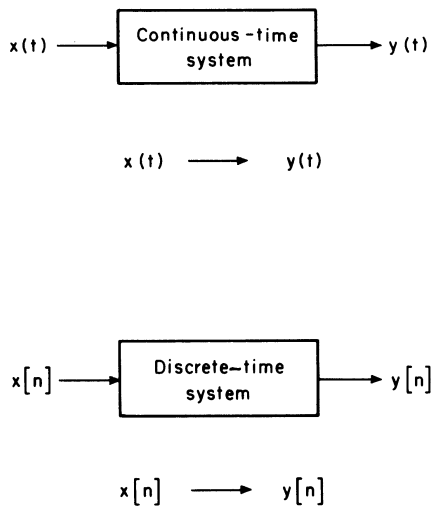
\includegraphics[height=0.8\textheight]{img/02.slide_09}
	\end{figure}
\end{frame}

\section{Interkoneksi Antar Sistem}

\begin{frame}{Interkoneksi Antar Sistem}
	\begin{figure}
		\centering
		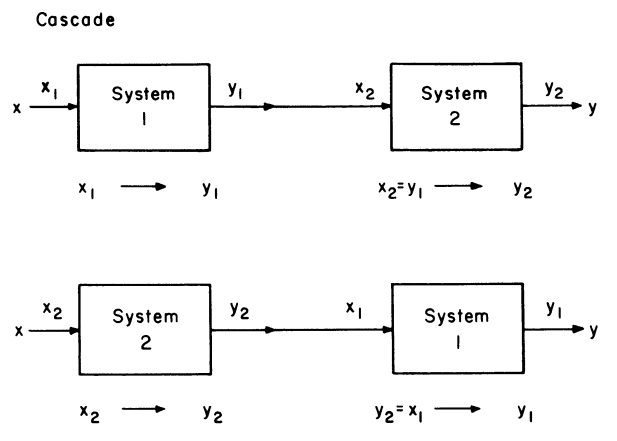
\includegraphics[height=0.8\textheight]{img/02.slide_10}
	\end{figure}
\end{frame}

\begin{frame}{Interkoneksi Antar Sistem}
	\begin{figure}
		\centering
		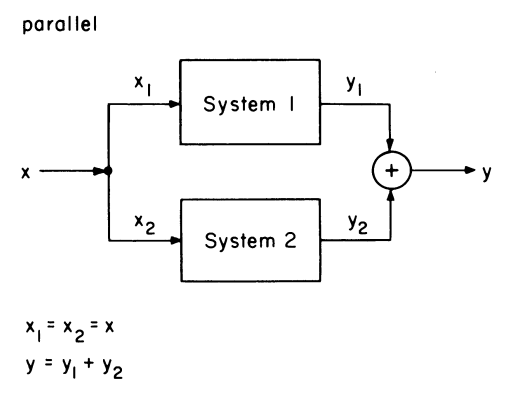
\includegraphics[height=0.8\textheight]{img/02.slide_11}
	\end{figure}
\end{frame}

\begin{frame}{Interkoneksi Antar Sistem}
	\begin{figure}
		\centering
		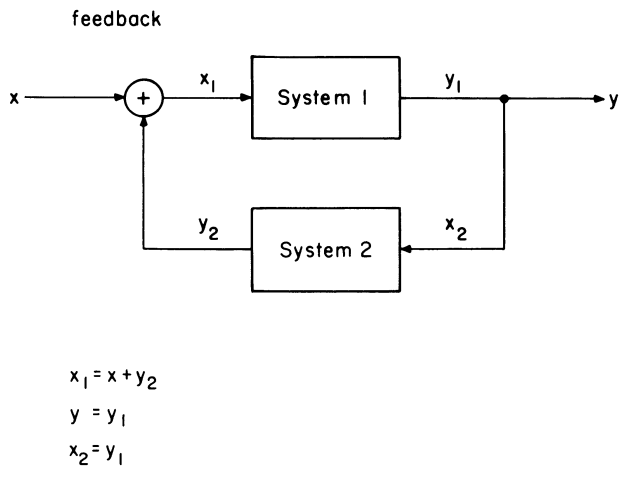
\includegraphics[height=0.8\textheight]{img/02.slide_12}
	\end{figure}
\end{frame}

\section{Karakteristik Sistem}

\begin{frame}
	\frametitle{Karakteristik Sistem}
	\begin{enumerate}
		\item Memoryless
		\item Invertibility
		\item Causality
		\item Stability
		\item Time Invariance
		\item Linearity
	\end{enumerate}
\end{frame}

\begin{frame}
	\frametitle{Memoryless}
	\textbf{Definition:} Output at any given time, $ t_0 $,  depends only on the input at the same time.
	\begin{align*}
		y(t); t=t_0 &\leftarrow x(t); t = t_0 \\
		y[n]; n=n_0 &\leftarrow x[n]; n = n_0
	\end{align*}
\end{frame}

\begin{frame}{Memoryless}
	Examples:
	\begin{enumerate}
		\item Squarer system $\rightarrow$ \textbf{Memoryless}
		\begin{align*}
		y(t) &= x^2(t) \\
		y[n] &= x^2[n]
		\end{align*}
		\item Integrator system $\rightarrow$ integrating the input $\rightarrow$ the value of the output at any time is an accumulation of past history of the input $\rightarrow$ \textbf{Not memoryless}
		\begin{align*}
		y(t) = \int_{-\infty}^{t} x^2(\tau)d\tau
		\end{align*}
	\end{enumerate}
\end{frame}

\begin{frame}{Memoryless}
	\begin{enumerate}
		\setcounter{enumi}{2}
		\item Unit delay $\rightarrow$ delay requires memory $\rightarrow$ \textbf{Not memoryless}
		\begin{align*}
			y[n] &= x[n-1]
		\end{align*}
	\end{enumerate}
\end{frame}

\begin{frame}
	\frametitle{Invertibility}
	\begin{itemize}
		\item \textbf{Definition:} Given the output, you can figure out uniquely what the input was. \textbf{Or} given the output, there is only one input that could have caused that.
	\end{itemize}
	
	\begin{align*}
		x_1(t) \xrightarrow[\text{}]{\text{A}} y_1(t) \longrightarrow x_2(t) \xrightarrow[\text{}]{\text{B}} y_2(t) \\
		x_1[n] \xrightarrow[\text{}]{\text{A}} y_1[n] \longrightarrow x_2[n] \xrightarrow[\text{}]{\text{B}} y_2[n]
	\end{align*}
	\begin{itemize}
		\item[] Note that $ x_2 = y_1 $
		\item If system A is invertible and system B is inverse of A, then $ y_2 = x_1 $
		\item \textbf{Identity system}: a system which if you put a signal into it, you get the same signal out of it
	\end{itemize}
\end{frame}

\begin{frame}{Invertibility}
	\textbf{Examples:}
	\begin{enumerate}
		\item System A: Integrator system $\rightarrow$ \textbf{Invertible}
		\begin{align*}
			y_1(t) = \int_{-\infty}^{t} x_1 (\tau) d\tau
		\end{align*}
		\item System $ \text{A}^{-1} $: Differentiator $\rightarrow$ \textbf{Invertible}/ \textbf{Not invertible}?
		\begin{align*}
			y_2(t) = \frac{dx_2(t)}{dt}
		\end{align*}
		$ \frac{d(3)}{dt} = 0 $ or $ \frac{d(7)}{dt} = 0 $. \textbf{Think about it's inverse!}
	\end{enumerate}
\end{frame}

\begin{frame}{Invertibility}
	\textbf{Examples:}
	\begin{enumerate}
		\setcounter{enumi}{2}
		\item System A: Squarer system $\rightarrow$ \textbf{Memoryless} but \textbf{Not invertible}
		\begin{figure}
			\centering
			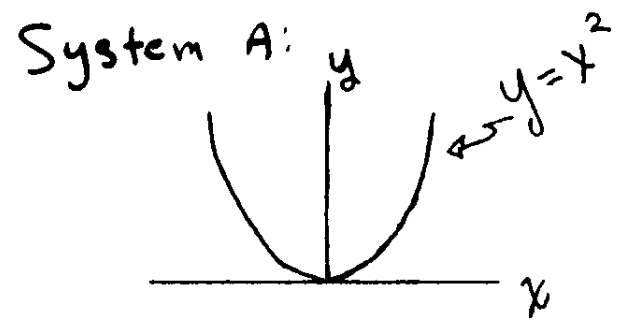
\includegraphics[height=0.3\textheight]{img/img01}
		\end{figure}
		\begin{align*}
			x = 2 \xrightarrow[\text{}]{\text{A}} y = 4 \\
			x = -2 \xrightarrow[\text{}]{\text{A}} y = 4
		\end{align*}
	\end{enumerate}
\end{frame}

\begin{frame}
	\frametitle{Causality}
	\textbf{Definition:} output at any time depends only on input prior or equal to that time, that means \textbf{system can't anticipate "future" inputs}
	\begin{align*}
		x_1(t) \longrightarrow y_1(t) \\
		x_2(t) \longrightarrow y_2(t)
	\end{align*}
	If: $ x_1(t) = x_2(t);~t<t_0$, then: $ y_1(t) = y_2(t);~t<t_0 $\\
	Same for discrete time
\end{frame}

\begin{frame}{Causality}
	\textbf{Examples:} Moving average system\\
	$ y[n] = \frac{1}{3}\{ x[n-1] + x[n] + x[n+1] \} \longrightarrow$ \textbf{Not causal}
	\begin{figure}
		\centering
		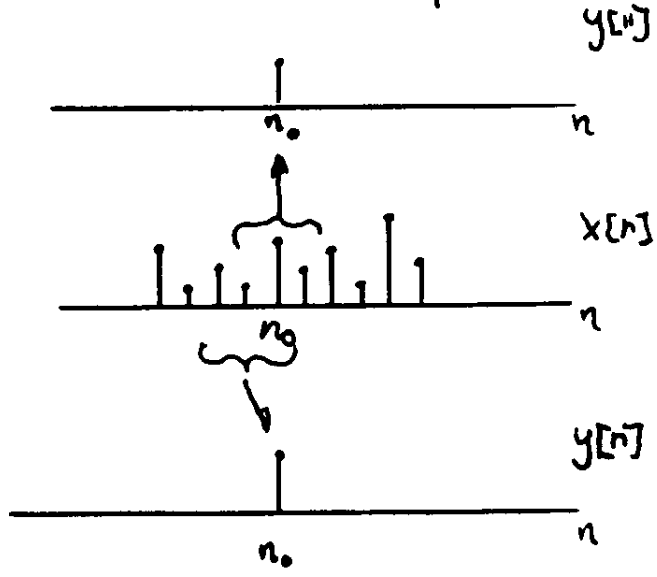
\includegraphics[height=0.5\textheight]{img/img02}
	\end{figure}
	$ y[n] = \frac{1}{3}\{ x[n-2] + x[n-1] + x[n] \} \longrightarrow $ \textbf{Causal}
\end{frame}

\begin{frame}
	\frametitle{Stability}
	\textbf{Definition:} Sistem is stable for every bounded input, the ouput is bounded
	\textbf{Examples:}
	\begin{enumerate}
		\item Integrator system: $ y(t) = \int\limits_{-\infty}^{t} x(\tau) d\tau $
		\begin{figure}
			\centering
			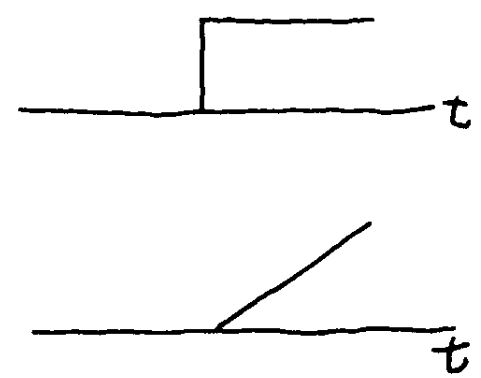
\includegraphics[height=0.3\textheight]{img/img03}
		\end{figure}
		The input is bounded but the output is not bounded $\longrightarrow$ \textbf{Not stable}
	\end{enumerate}
\end{frame}

\begin{frame}
	\frametitle{Time invariance}
	\textbf{Definition:}
	\begin{itemize}
		\item Cont. Time.\\
		If $ x(t) \longrightarrow y(t) $ then $ x(t-t_0) \longrightarrow y(t-t_0) $
		\item Dis. Time.\\
		If $ x[n] \longrightarrow y[n] $ then $ x[n-n_0] \longrightarrow y[n-n_0] $
	\end{itemize}
\end{frame}

\begin{frame}{Time invariance}
	\textbf{Examples:}
	\begin{enumerate}
		\item Accumulator system $ \longrightarrow $ \textbf{Time invariant}
		\begin{align*}
			y[n] = \sum_{k=-\infty}^{n}x[k]
		\end{align*}
		\item $ y(t) = (\sin(t)) x(t) $ $\longrightarrow$ \textbf{Not time invariant}
		\begin{align*}
			x(t) & \rightarrow (\sin (t)) x(t) \\
			x(t-t_0) & \rightarrow (\sin (t)) x(t-t_0) \\
			y(t-t_0) & \rightarrow (\sin (t-t_0)) x(t-t_0) \\
			(\sin (t)) x(t-t_0) & \neq (\sin (t-t_0)) x(t-t_0) \\
		\end{align*}
	\end{enumerate}
\end{frame}

\begin{frame}
	\frametitle{Linearity}
	Cont. Time \& Dis. Time\\
	\textbf{Definition:}\\
	\begin{itemize}
		\item[] \textbf{If:}
		\begin{align*}
		x_1(t) &\rightarrow y_1(t) \\
		x_2(t) &\rightarrow y_2(t) \\
		\end{align*}
		\textbf{Then:}
		\begin{align*}
		ax_1(t) + bx_2(t) \rightarrow ay_1(t) + by_2(t)
		\end{align*}
		linear combination input $\rightarrow$ linear combination output
	\end{itemize}
\end{frame}

\begin{frame}{Linearity}
	\textbf{Examples:}
	\begin{enumerate}
		\item Linear
		\begin{align*}
			y(t) = \int_{-\infty}^{t} x(\tau)d\tau
		\end{align*}
		\item Not linear\\
		\begin{align*}
			y[n] = 2x[n]+3
		\end{align*}
		Linear = zero input $\rightarrow$ zero output. But $ x[n] = 0 \rightarrow y[n] = 2\cdot0 + 3 = 3 \rightarrow$ \textbf{Not linear}
		\item Not linear
		\begin{align*}
			y[n] = x^2[n]
		\end{align*}
	\end{enumerate}
\end{frame}

\begin{frame}
	\frametitle{Tugas Mandiri}
	\begin{enumerate}
		\item Oppenheim, A. V., Willsky, A. S. \& Nawab, S. H., (1997). Signal and Systems, Second Edition. New Jersey: Prentice Hall of India.
		\begin{itemize}
			\item Section 1.1, Transformations of the independent variable, pp. 7-11
			\item Section 1.3.1, Continuous-time complex exponential and sinusoidal signals, pp. 15-21
			\item Section 1.3.2, Discrete-time complex exponential and sinusoidal signals, pp. 21-25
			\item Section 1.3.3, Periodicity properties of discrete-time complex exponentials, pp. 25-30
		\end{itemize}
	\end{enumerate}
\end{frame}

\begin{frame}
	\frametitle{Tugas Terstruktur}
	\textbf{Tampilkan Tugas 1}
\end{frame}

\end{document}
